\documentclass{article}


\usepackage{lipsum}
\usepackage[margin=1in,includefoot]{geometry}
\usepackage{graphicx}
\usepackage{float}
\usepackage[hidelinks]{hyperref}
\usepackage{amsmath}
\usepackage{amssymb}
\usepackage{color}
\usepackage[english]{babel}
\usepackage{subcaption}

\usepackage{booktabs}
\usepackage[normalem]{ulem}
\useunder{\uline}{\ul}{}

\usepackage[usenames,dvipsnames]{xcolor}
\usepackage{listings}


% Header and Footer Stuff
\usepackage{fancyhdr}
\pagestyle{fancy}
\fancyhead{}
\fancyfoot{}
\fancyfoot[R]{\thepage}
\renewcommand{\headrulewidth}{0pt}
\renewcommand{\footrulewidth}{0pt}




\definecolor{dkgreen}{rgb}{0,0.6,0}
\definecolor{gray}{rgb}{0.5,0.5,0.5}
\definecolor{mauve}{rgb}{0.58,0,0.82}


\lstset{
 language=C++,
 aboveskip=3mm,
 belowskip=3mm,
 showstringspaces=false,
 columns=flexible,
 basicstyle={\small\ttfamily},
 numbers=none,
 numberstyle=\tiny\color{gray},
 keywordstyle=\color{blue},
 commentstyle=\color{dkgreen},
 stringstyle=\color{mauve},
 breaklines=true,
 breakatwhitespace=true,
 tabsize=3
}




\begin{document}


\begin{titlepage}
	\begin{center}
	\begin{align*}
	
\includegraphics[height=1.75in]{logo.png}
	\end{align*}




	
	\line(1,0){300}\\
	[0.25in]
	\huge{\bfseries Door Detection}\\
	[2mm]
	\line(1,0){200}\\
	[1.5cm]
	\textsc{\LARGE Assignment 2}\\
	[0.75cm]
	\textsc{\Large CS4053 Computer Vision}\\
	[7cm]	
	\end{center}
	
	
	
	\begin{flushright}
	\textsc{\large Alexandru Sulea\\
	D Stream\\
	\#12315152\\
	13 December 2016\\}
	\end{flushright}
	
\end{titlepage}
%Table of Contents Stuff%
\tableofcontents
%\listoffigures
%\addcontentsline{toc}{section}{List of Figures}
\listoftables
\addcontentsline{toc}{section}{List of Tables}




\thispagestyle{empty}
\cleardoublepage
\pagenumbering{arabic}
\setcounter{page}{1}


\pagebreak
\section{RED PIXEL DETECTION}
\subsection{Intro}\label{sec:intro}
The following lab was based on the procedure of determining when a door is opened and closed in a room given that there is a person walking through the door and that the light in the scene can vary depepnding on the lighting conditions in the room but also from the light propagating in the scene from the hallway.\\
Unlike the previous lab, this required a mixture of different procedures all acting at the same time so as to not only remove potential error inducing details but to also improve the accuracy of the door opening.\\

\begin{lstlisting}




\end{lstlisting}
\subsection{Procedure}\label{sec:intro}
Taking notes of what was discussed and shown in class together with the theory and description on the official opencv page, the following procedure was planned out. 
The scene itself consists of two distinct parts. The first being a man walking from foreground to background and back, the second being that a door opens and closes at arbitrary intervals. The person in the picture serves no real purpose for this lab other than to induce uncertainty of when the door opens and closes. Thus the first operation is to perform a background subtraction on the person and have them removed as much as possible from the scene. This will not only allow us to see the door more clearly, but it will also help clean up the frames and make Hough Lines more accurate later on.\\


Once the person is removed from the picture, the door detection must begin.\\ Here a number of already built in opencv procedures can be used such as HoughLines() , HoughLineP() or SNP. Although SNP is somewhat more accurate then HoughLineP(), the later is also more easily custamizable and faster to process. Given how door frame tracking throughout every video frame was not the objective and only opening and closing, HoughLineP was chosen to help with the door detection. \\
Here whatever lines were detected in the scene by houghlinesP, only the lines that were horizontal or vertical, given 10 degrees of error were accepted as the true vertical and horizontal lines.\\
After the horizontal and vertical lines were filtered through, their deterinates are calculated and compared to all the other vertical or horizontal lines as to check if the lines form a box at any point. Should the lines intersect, a circle is drawn at the intersection points.




\begin{figure}[H]
\begin{subfigure}{0.5\textwidth}

\includegraphics[width=0.9\linewidth, height=5cm]{ROADSIGN_samplered.png} 
\caption{The second last red sample}
\label{fig:subim1}
\end{subfigure}
\begin{subfigure}{0.5\textwidth}

\includegraphics[width=0.9\linewidth, height=5cm]{ROADSIGN_samplered2.png}
\caption{The red sample image used for the current results}
\label{fig:subim2}
\end{subfigure}
\caption{Figure of constructed red sample images}
\label{fig:image2}
\end{figure}
Thus, a new sample red image had to be created to make a histogram which would only contain the red present in road signs. To make the red sample image  the photoshop program gimp was used to make a simple grid in which different red hues were stored. The red hue samples were taken from the sample road signs image. The images road signs were sampled at different points so as to get an even, accurate representation of the red color used in the road signs.\\
Once the new sample red image had been created using different points on road signs in the sample road signs image the code could finally be written in.\\
The first step is to load in the images and check that the correct images have been loaded by the program without any exceptions or errors being thrown. That is where this part of the code comes in.
\begin{lstlisting}
Mat roadsign_test2 = imread("filename.JPG", CV_LOAD_IMAGE_UNCHANGED);
if (roadsign_sample.empty()){
		printf("Cannot open video file: \n");
		return -1;}
	else { ...}
\end{lstlisting}
Next the image is converted to HSV or Hue Saturation Value so that we can separate the hue from the rest of the image. Since we are only interested in the color red and its multiple shades we will only be using hue, thus creating a 1D Red Hue Histogram.


\begin{lstlisting}
//hue is from 0 to 180
		float huerange[] = {0, 180};
		//use only hue value
		hue_red.create(hsv_sample_red.size(), hsv_sample_red.depth());
		mixChannels(&hsv_test, 1, &hue_test, 1, ch, 1);
		/*Calculate and Normalize Hist*/
		calcHist(&hue_red, 1, ch, Mat(), hist_red, 1, &histSize_red, &ranges, true, false);
		normalize(hist_red, hist_red, 0, 255, NORM_MINMAX, -1, Mat());
		//drawing out the red histogram
		Mat histImg = Mat::zeros(w, h, CV_8UC3);
		for (int i = 0; i < bins; i++)
		{
			rectangle(histImg, Point(i*bin_w, h), Point((i + 1)*bin_w, h - cvRound(hist_red.at<float>(i)*h / 255.0)), Scalar(0, 0, 255), -1);}
		calcBackProject(&hue_test, 1, 0, hist_red, backproj, &ranges, 1, true);	
		threshold(backproj, thresh_backproj, 8, 255, CV_THRESH_BINARY);
		dilate(thresh_backproj, dil_thresh_backproj, Mat(), Point(-1, -1), 2, 1, 1);
\end{lstlisting}


To preserve the traffic sign shapes in the image throughout the contour hierarchy process the final red pixel detection process was altered to allow for the black and white pixel detection later on.\\
\begin{figure}[H]
\begin{subfigure}{0.5\textwidth}
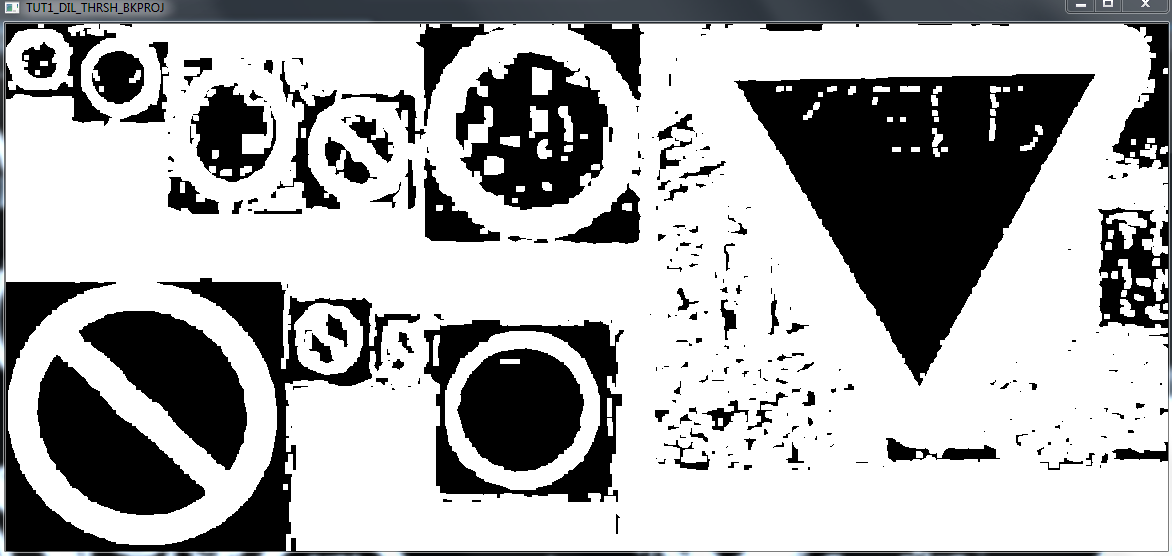
\includegraphics[width=0.9\linewidth, height=5cm]{N_DIL_THRESH_BKPROJ.PNG} 
\caption{The back projected image}
\label{fig:subim1}
\end{subfigure}
\begin{subfigure}{0.5\textwidth}

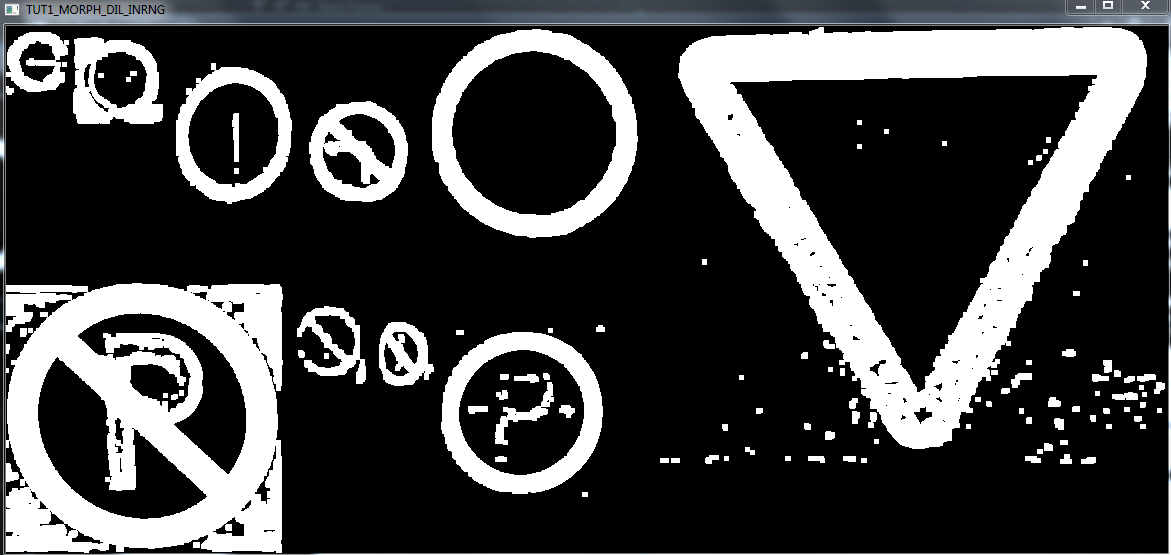
\includegraphics[width=0.9\linewidth, height=5cm]{N_MORPH_DIL_INRNG.PNG}
\caption{The inRange thresholded image}
\label{fig:subim2}
\end{subfigure}
\caption{Figure of constructed tresholded images}
\label{fig:image2}
\end{figure}

\begin{figure}[H]
\center
\begin{subfigure}{0.5\textwidth}
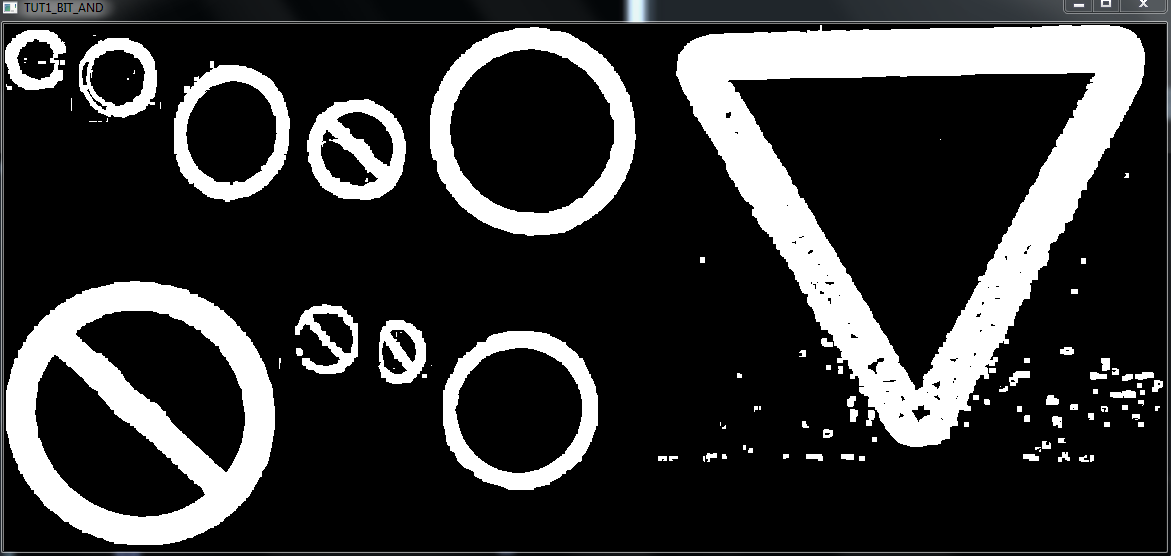
\includegraphics[width=0.9\linewidth, height=5cm]{N_BIT_AND.PNG} 
\caption{The two images above ANDed give this result}
\label{fig:subim1}
\end{subfigure}
\caption{Figure of constructed of the two tresholded images}
\label{fig:image2}
\end{figure}


\begin{lstlisting}
		inRange(hls_test, Scalar(10,10,55), Scalar(210, 190, 200), inrange_test);
		dilate(inrange_test, dil_inrange_test, Mat(), Point(-1, -1), 2, 1, 1);
		// Two images, back proj and inrange merged together
		bitwise_and(dil_thresh_backproj, morph_dil_inrange_test, band_rng_bkprj);
		dilate(band_rng_bkprj, band_rng_bkprj, Mat(), Point(-1, -1), 1, 1, 1);
		/*Dilate and morphology again to close the remaining gaps*/
		morphologyEx(band_rng_bkprj, band_rng_bkprj, MORPH_TOPHAT, element, Point(-1, -1), 50);
		bitwise_and(roadsign_test,roadsign_test,redcrop, band_rng_bkprj);
\end{lstlisting}


\begin{figure}[H]
\begin{subfigure}{0.5\textwidth}
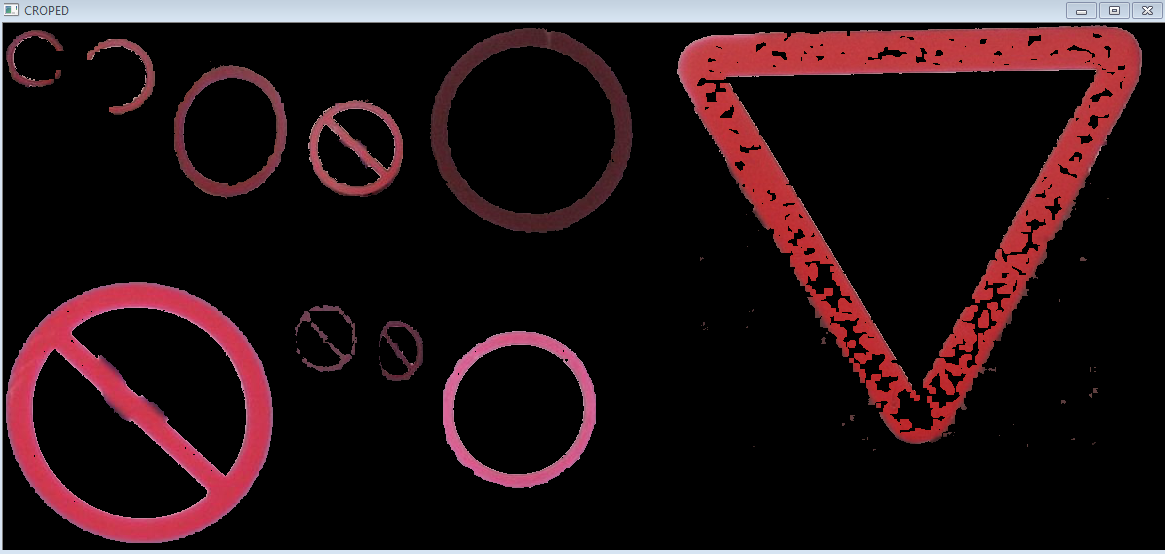
\includegraphics[width=0.9\linewidth, height=5cm]{CROPP.PNG} 
\caption{A previous, less succesfull composite image using the previous $($a$)$ red sample image}
\label{fig:subim1}
\end{subfigure}
\begin{subfigure}{0.5\textwidth}
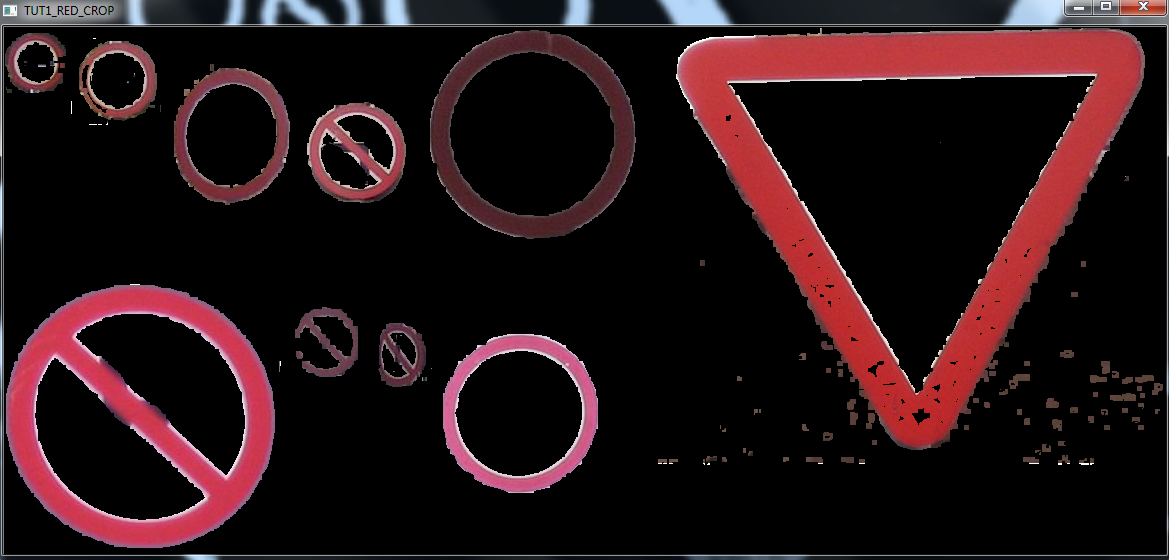
\includegraphics[width=0.9\linewidth, height=5cm]{N_RED_CROP.PNG}
\caption{The composite image showing the current red mixels detected}
\label{fig:subim2}
\end{subfigure}
\caption{Figure of constructed tresholded images}
\label{fig:image2}
\end{figure}




\begin{lstlisting}
CompareRecognitionResults(band_rng_bkprj, ground_red);
\end{lstlisting}
The above code shows the use of the function CompareRecognitionResults to compare the example thresholded red pixel image with the thresholded ground pixel image to achieve a score for the performance method. \\
The ground image is converted to HLS and then used inRange on it as discussed before. The only difference to this is that the ground image has only one overall value for each color present, making it very easy to threshold out the colors. Thus the following code was used to get the ground thresholded images of the three colors.
\begin{lstlisting}
	inRange(hls_ground, Scalar(0, 0, 255), Scalar(0, 0, 255), ground_white);
	inRange(hls_ground, Scalar(0, 255, 255), Scalar(0, 255, 255), ground_red);
	inRange(hls_ground, Scalar(0, 0, 0), Scalar(0, 0, 0), ground_black);
\end{lstlisting}
%\includegraphics[height=2in,width=5in]{}
%\includegraphics[height=2in,width=5in]{}




\subsection{Performance}\label{sec:intro}
Given as how the ground truth was provided or this lab in terms of door frame position and opening and closing frames, it was quite simple to compare the achieved results to the ground truth. \\





\begin{figure}[H]
\center
\begin{subfigure}{0.5\textwidth}
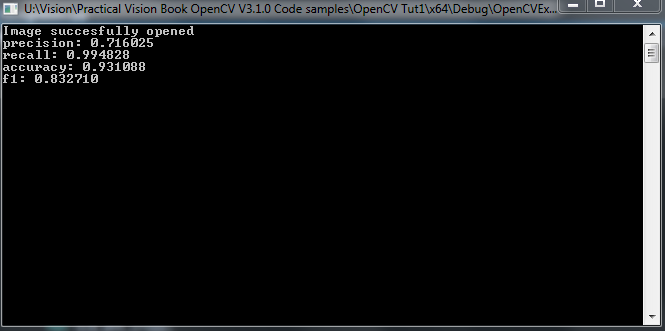
\includegraphics[width=0.9\linewidth, height=4cm]{N_RED_STAT.PNG} 
\caption{The image shows the scoring achieved for the red pixels}
\label{fig:subim2}
\end{subfigure}
\caption{The figure shows the scores for red pixel recognition}
\label{fig:image2}
\end{figure}

\begin{table}[]
\centering
\caption{RED PIXEL DETECTION VALUES}
\label{my-label}
\begin{tabular}{@{}|l|l|@{}}
\toprule
{\ul TYPE} & {\ul VALUE} \\ \midrule
Precision  & 0.716025    \\ \midrule
Recall     & 0.994828     \\ \midrule
Accuracy   & 0.931088    \\ \bottomrule
\end{tabular}
\end{table}


\subsection{Discussion}\label{sec:intro}
While solving the problems inherent in detecting a door, a number of problems arose. The main being that, even though the solution was designed to fit a wide array of cases, it will fail in many more due to a variety of problems such as:

\begin{enumerate}
	\item The precision and accuracy of the solution is heavily depepndent of the lighting conditions present and also the color difference of the door as oposed to its background.\\ While doing the lab, the algorythms continuily had problems detecting where the door ended and the door frame ended, due to the fact that the two were very flush and of the same design and color.
	\item The door shape itself would need to have 4 corners to provide an accurate door representation, any lift doors or star trek/ star wars type doors would not be detected. Thus leading humanity to be vulnerable to attack :)
\end{enumerate}











\pagebreak
\end{document}


